\documentclass[xcolor=dvipsnames]{beamer}
\mode<presentation>
{
  \usetheme{Darmstadt}
%  \usetheme{Szeged}
  \usefonttheme{professionalfonts}
  \setbeamerfont*{frametitle}{size=\normalsize,series=\bfseries}
  \setbeamertemplate{navigation symbols}{}
  \definecolor{UVABlue}{RGB}{0,47,108}
  \definecolor{UVAOrange}{RGB}{229,114,0}
  \usecolortheme[named=UVABlue]{structure}

  \setbeamercolor*{palette secondary}{use=structure,fg=white,bg=UVABlue}
%  \setbeamercolor*{palette tertiary}{use=structure,fg=white,bg=UVABlue}
  \setbeamercolor*{block title}{use=structure,fg=white,bg=UVABlue}
  \setbeamercolor*{block title example}{use=structure,fg=white,bg=UVAOrange}
  \setbeamercolor*{block body example}{use=structure,bg=white}
  }
\usepackage{amsmath} \usepackage{amssymb} \usepackage{amsfonts}
\usepackage{amsthm} \usepackage{enumerate} \usepackage[all]{xy}
\usepackage{ulem}
\usepackage{tikz-cd}
\usetikzlibrary{decorations.markings,arrows}

\beamertemplateballitem

\mode<presentation>
{
  \usetheme{Warsaw}
%\usecolortheme[named=OliveGreen]{structure}
  \setbeamercovered{transparent}
}

\usepackage[english]{babel}
\usepackage[latin1]{inputenc}
\usepackage{times}
\usepackage[T1]{fontenc}


\def\souta{\bgroup \ULdepth=-.7ex \ULset}


\newcommand{\Z}{\mathbb{Z}}
\newcommand{\R}{\mathbb{R}}
\newcommand{\C}{\mathbb{C}}
\newcommand{\sC}{\mathcal{C}}
\newcommand{\Q}{\mathbb{Q}}
\newcommand{\E}{\mathbb{E}}
\renewcommand{\S}{\mathbb{S}}
\newcommand{\cA}{\mathcal{A}}
\newcommand{\cM}{\mathcal{M}}
\newcommand{\cE}{\mathcal{E}}
\newcommand{\cp}{\mathcal{p}}
\newcommand{\otfr}{\otimes_{F(R)}}
\newcommand{\otr}{\otimes_R}
\newcommand{\KK}{\mathbb{K}}
\newcommand{\kk}{\mathbbm{k}}
\newcommand{\otzg}{\otimes_{\Z[G]}}
\newcommand{\ot}{\otimes}
\newcommand{\bphi}{\bar{\phi}}
\newcommand{\bpsi}{\bar{\psi}}
\newcommand{\FF}{\mathbb{F}}
\newcommand{\LL}{\mathbb{L}}
\newcommand{\Cay}{\mathrm{Cay}}
\newcommand{\CAT}{\mathrm{CAT}}
\newcommand{\lk}{\mathrm{lk}}
\newcommand{\geom}{\mathrm{geom}}
\newcommand{\rhob}{\bar{\rho}}
\newcommand{\inte}{\mathrm{int}}
\newcommand{\cS}{\mathcal{S}}
\newcommand{\cG}{\mathcal{G}}
\newcommand{\Stab}{\mathrm{Stab}}
\newcommand{\SL}{\mathrm{SL}}
\newcommand{\FP}{\mathrm{FP}}
\newcommand{\normal}{\trianglelefteq}
\newcommand{\bZ}{\bar{Z}}


\newtheorem{Ques}{Question}
\newtheorem{Theo}{Theorem}
\newtheorem{Prop}{Proposition}
\newtheorem{Cor}[Theo]{Corollary}
\newtheorem{Conj}[Theo]{Conjecture}
\newtheorem{Lem}[Theo]{Lemma}
\theoremstyle{definition}
\newtheorem{Defn}[Theo]{Definition}
\newtheorem{Exam}[Theo]{Example}



\def\adots{\mathinner{\mkern2mu\raise0pt\hbox{.}  % antidiagonal dots
\mkern2mu\raise4pt\hbox{.}\mkern1mu
\raise7pt\vbox{\kern7pt\hbox{.}}\mkern1mu}}

\title[Finite Presentability of Groups Acting on Twin Buildings]{Finite Presentability of Groups Acting on Locally Finite Twin Buildings}
\author{Zachary Gates}
\institute{Department of Mathematics\\University of Virginia}

\date{April 19, 2018}

\subject{Talks}

% If you have a file called "university-logo-filename.xxx", where xxx
% is a graphic format that can be processed by latex or pdflatex,
% resp., then you can add a logo as follows:

% \pgfdeclareimage[height=0.5cm]{university-logo}{university-logo-filename}
% \logo{\pgfuseimage{university-logo}}


% Delete this, if you do not want the table of contents to pop up at
% the beginning of each subsection:
% \AtBeginSubsection[]
% {
%   \begin{frame}<beamer>{Outline}
%     \tableofcontents[currentsection,currentsubsection]
%   \end{frame}
% }

\begin{document}


\begin{frame}
  \titlepage
\end{frame}



%\begin{frame}
%\frametitle{What are Kac-Moody groups?}
%\begin{itemize}
%\item They are infinite-dimensional generalizations to semi-simple linear algebraic groups.
%
%\item Each Kac-Moody group has an associated Weyl group (a Coxeter group), which will be how we classify them in order to study their finiteness properties.
%\item Example: $\SL_n(\FF_q[t, t^{-1}])$ is an affine Kac-Moody group of type $\tilde{A}_{n-1}$.
%\item Twin buildings arose as a geometric way to study these groups.
%\end{itemize}
%\end{frame}

\begin{frame}
\frametitle{Coxeter systems}
\begin{Defn}
A \textit{Coxeter system} is a pair $(W,S)$ consisting of a group $W$ and generating set $S$ such that $W$ admits a presentation $W = \langle S | (st)^{m(s,t)}=1\text{ for all }s,t\in S\rangle$, where $m(s,t)\in \mathbb{N}\cup \{\infty\}$, $m(s,t) = m(t,s)$, and $m(s,t) = 1$ if and only if $s=t$ for all $s,t\in S$. In fact, $m(s,t)$ is the order of $st$, and $m(s,t)=\infty$ means there are no relations.
\end{Defn}
\smallskip

Some examples:
\begin{itemize}
\item The dihedral group $D_{2n} =  \langle s, t| s^2 = t^2 = (st)^n = 1 \rangle$
\item The infinite dihedral group $D_{\infty} = \langle s,t| s^2 = t^2 = 1\rangle$
\item The symmetric group $$S_n = \langle s_1,\ldots, s_{n-1}|s_i^2 = 1, (s_i s_{i+1})^3 =1, (s_i s_j)^2 = 1\text{ if } |i-j|> 1\rangle$$
\end{itemize}

\end{frame}

\begin{frame}
\frametitle{The Coxeter diagram}
We can associate a Coxeter diagram to a Coxeter group by assigning a node for each generator and putting an edge between two vertices $i$ and $j$ if $m_{ij}\geq 3$ and labeling that edge with $m_{ij}$ if $m_{ij}>3$.

\vskip .5cm

$D_{2n}$:
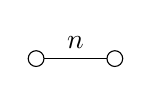
\begin{tikzpicture}
\draw (0,0) circle (.1);
\draw (1,0) circle (.1);
\draw (.1,0)-- (.9,0) node[above, pos = .5]{$n$};
\end{tikzpicture}
\vskip .5cm

$D_{\infty}$:
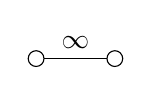
\begin{tikzpicture}
\draw (0,0) circle (.1);
\draw (1,0) circle (.1);
\draw (.1,0)-- (.9,0) node[above, pos = .5]{$\infty$};
\end{tikzpicture}

\vskip .5cm
$W = \langle s_1, s_2, s_3 | s_1^2 = s_2^2 = s_3^2 = (s_1 s_2)^3 = (s_2 s_3)^4 = (s_1 s_3)^2 = 1\rangle$:
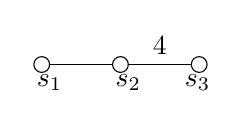
\begin{tikzpicture}
\draw (0,0) circle (.1);
\draw (1,0) circle (.1);
\draw (2,0) circle (.1);
\draw (.1,0) - - (.9,0) node[below,pos=0]{$s_1$};
\draw (1.1,0) - - (1.9,0) node[above, pos = .5]{$4$} node[below, pos=1.1]{$s_3$} node[below, pos=0]{$s_2$};
\end{tikzpicture}

\end{frame}

\begin{frame}
\frametitle{Coxeter complexes}
\begin{itemize}
\item A \textit{Coxeter complex} of type $(W,S)$ is a simplicial complex associated to a Coxeter system $(W,S)$. Its dimension is $|S|-1$.
\vskip .3cm 
\item The \textit{chambers} (maximal dimension simplices) are in 1-1 correspondence with elements of $W$.
\vskip .3cm
\item The codimension-$1$ simplices are called \textit{panels} and can be labeled with elements of $S$. If two chambers share an $s$-panel for some $s\in S$, they are called \textit{$s$-adjacent}.
\vskip .3cm
\item If $W$ is finite, the Coxeter complex is homeomorphic to a $(|S|-1)$-sphere. In this case, we say $(W,S)$ is a \textit{spherical} Coxeter system.
\end{itemize}
\end{frame}

\begin{frame}
\frametitle{Examples}
\begin{flushleft}
$\tilde{A}_2$
\includegraphics[height=1.2in]{affineA2.png}
\end{flushleft}


\begin{flushright}
$A_2$
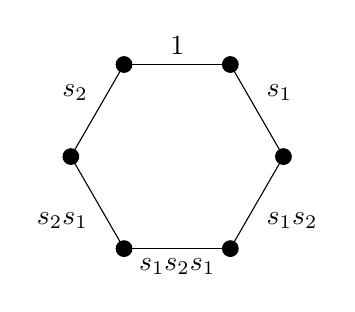
\begin{tikzpicture}[scale = .5]
\newdimen\R
  \R=2.7cm
  \foreach \x/\l in
    { 60/$s_1$,
     120/$1$,
     180/$s_2$,
     240/$s_2s_1$,
     300/$s_1s_2s_1$,
     360/$s_1s_2$
    }
    \draw[postaction={decorate}] ({\x-60}:\R) -- node[auto,swap]{\l} (\x:\R);
  \foreach \x/\l/\p in
    { 60/{}/above,
     120/{}/above,
     180/{}/left,
     240/{}/below,
     300/{}/below,
     360/{}/right
    }
    \node[inner sep=2pt,circle,draw,fill,label={\p:\l}] at (\x:\R) {};
\end{tikzpicture}
%\includegraphics[height=1in]{A2Coxeter.png}
\end{flushright}


\end{frame}

\begin{frame}
\frametitle{Buildings and Twin Buildings}
\begin{itemize}
\item A building of type $(W,S)$ is a simplicial complex built out of Coxeter complexes of type $(W,S)$ satisfying certain axioms.\\
\vskip .2cm
Example: A tree without endpoints is a building of type $(D_{\infty}, \{s,t\})$.
\begin{center}
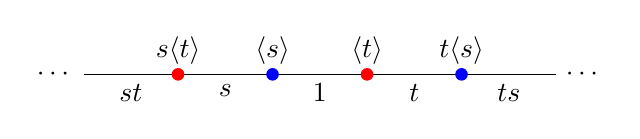
\begin{tikzpicture}[scale = .8]
\draw (-1.5,0) -- (0,0) node[left, pos = 0]{$\cdots$} node[below, pos = .5]{$st$} node[above, pos = 1]{$s\langle t\rangle$} -- (1.5,0) node[below, pos = .5]{$s$}  node[above, pos = 1]{$\langle s\rangle$} -- (3,0) node[below, pos = .5]{$1$} node[above, pos = 1]{$\langle t\rangle$} -- (4.5,0) node[below, pos = .5]{$t$} node[above, pos = 1]{$t\langle s\rangle$} -- (6,0) node[below, pos = .5]{$ts$} node[right, pos = 1]{$\cdots$};
\fill[red] (0,0) circle (.1);
\fill[blue] (1.5,0) circle (.1);
\fill[red] (3,0) circle (.1);
\fill[blue] (4.5,0) circle (.1);
\end{tikzpicture}
\end{center}
\vskip .4cm
\item A twin building of type $(W,S)$ is a pair of buildings of the same type with an opposition relation between them. These generalize spherical buildings.
\vskip .4cm
\item The theory of twin buildings was developed by Tits and Ronan to study Kac-Moody groups, which naturally act on twin buildings.
\end{itemize}
\end{frame}

\begin{frame}
\frametitle{Kac-Moody groups}
\begin{itemize}
\item These can be thought of as infinite-dimensional analogues of semisimple Lie groups.
\vskip .6cm

\item Any Kac-Moody group has an associated Weyl group $W$ and hence Coxeter system $(W,S)$.
\vskip .6cm

\item Example: $\SL_n(\FF_q[t, t^{-1}])$ is an affine Kac-Moody group of type $\tilde{A}_{n-1}$ over $\FF_q$.
\vskip .6cm

\item The key structure we gain from a strongly transitive action on a twin building is a \textit{twin BN-pair}.
\end{itemize}

\end{frame}

\begin{frame}
\frametitle{What is known about Kac-Moody groups?}
\begin{itemize}
\item Kac-Moody groups over infinite fields are always infinitely generated, and Kac-Moody groups over finite fields are always finitely generated.

\begin{Ques}
When are Kac-Moody groups over finite fields finitely presented?
\end{Ques}

\item Abramenko and M{\"u}hlherr showed that $\cG(\FF_q)$ is finitely presented in the $2$-spherical case (all finite labels in Coxeter diagram).
\item Stuhler showed that $\SL_2(\FF_q[t,t^{-1}])$ is not finitely presented in 1980 using different methods.


\end{itemize}
\end{frame}



\begin{frame}
\frametitle{Conjecture}
\begin{Conj}
Let $G$ be a group acting strongly transitively on a locally finite twin building. If the Coxeter diagram for $G$ has an $\infty$ label, then $G$ is not finitely presented.
\end{Conj}

\end{frame}

\begin{frame}
\frametitle{Tools}
\begin{Defn}
A group is said to be $\FP_n$ if there is a projective resolution of $\Z$ by $\Z[G]$-modules $\cdots \to P_{n+1}\to P_n\to \cdots \to P_0 \to \Z$ such that $P_0, \ldots, P_n$ are finitely generated.
\end{Defn}

$\FP_1$ is equivalent to finite generation and finite presentation implies $\FP_2$.


\begin{Theo}[Gandini, 2012]
If a group acts cellularly on a product of two trees with finite stabilizers of unbounded order, then $G$ is not $\FP_2$. In particular, $G$ is not finitely presented.
\end{Theo}



\end{frame}

\begin{frame}
\frametitle{Tools}


\begin{Defn}[$Z$-realization of a building]
Let $Z$ be any topological space with a family of nonempty closed subsets $Z_s$ for each $s\in S$ and let $\Delta$ be a building. Then we define $Z(\Delta)$ as a quotient of $Z\times \sC$ where we glue copies of $Z$ together by their $s$-panels if the associated chambers are $s$-adjacent in the building.
\end{Defn}
\vskip 1cm
Idea: $Z$ is the model for a closed chamber and $Z_s$ is the $s$-panel. We want $Z(\Delta)$ to be a tree, so that we can apply Gandini's theorem.
\end{frame}

\begin{frame}

\frametitle{Examples of $Z$}
\begin{flushleft}
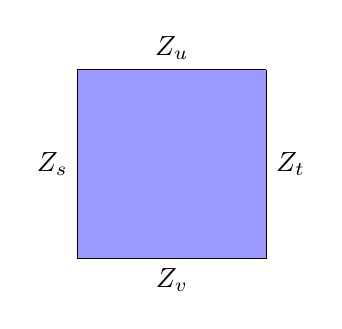
\begin{tikzpicture}[scale = .8]
\fill[fill=blue!40!white] (0,0) -- (3,0) -- (3,3)  -- (0,3);
\draw (0,0)--(3,0) node[pos = .5, below]{$Z_v$};
\draw (0,0) -- (0,3) node[pos = .5, left]{$Z_s$};
\draw (0,3)--(3,3) node[pos = .5, above]{$Z_u$};
\draw (3,0)--(3,3) node[pos = .5, right]{$Z_t$};
\end{tikzpicture}
\end{flushleft}



\begin{flushright}
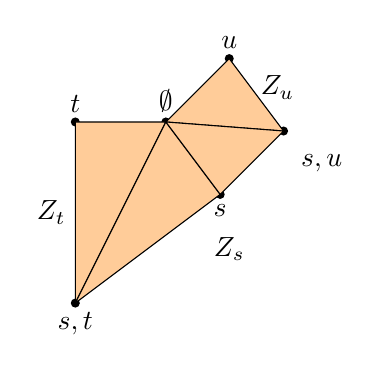
\begin{tikzpicture}[scale = 1.15]
\fill (0,0) circle (.05);
\fill (0,2) circle (.05);
\fill (1,2) circle (.05);
\filldraw[fill = orange!40] (0,0) - - (0,2) node[left, pos = .5]{$Z_t$} - - (1,2) node[above, pos = 0]{$t$} node[above, pos =1]{$\emptyset$} - - cycle;
\fill (1.6, 1.2) circle (.05);
\filldraw[fill = orange!40] (0,0) - - (1.6,1.2) node[below, pos = 0]{$s,t$} node[below, pos = 1]{$s$}  - - (1,2) - - cycle;
\fill (1.7, 2.7) circle (.05);
\fill (2.3, 1.9) circle (.05);
\filldraw[fill = orange!40] (1,2) - - (1.7,2.7) node[above, pos = 1]{$u$}- - (2.3,1.9) node[above, pos = 1.7]{$s,u$} node[right, pos =.4]{$Z_u$} - - cycle;
\filldraw[fill = orange!40] (1.6,1.2) - - (2.3, 1.9) - - (1,2) - - cycle;
\node at (1.7, .6){$Z_s$};

\end{tikzpicture}
\end{flushright}
\end{frame}



\begin{frame}
\frametitle{Davis Realization}
\begin{Defn}
The \textit{Davis realization} of a building is a specific case of the more general $Z$-realization where $Z$ is the geometric realization of the flag complex on the spherical subsets of $S$ and $Z_s$ is the geometric realization of the flag complex on the spherical subsets of $S$ containing $s$.
\end{Defn}

The Davis realization works if all labels are $\infty$ but will, in general, have too high dimension to apply Gandini's theorem.

\begin{center}
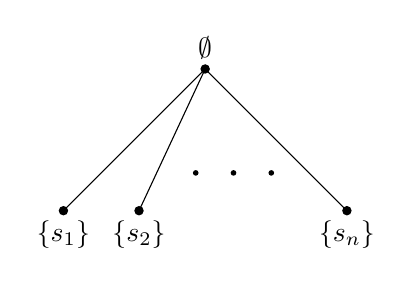
\begin{tikzpicture}[scale = .6]
\fill (0,0) circle (.1);
\fill (1.6,0) circle (.1);
\fill (6,0) circle (.1);
\fill (3,3) circle (.1);
\draw (3,3) - - (0,0) node[pos = 0, above]{$\emptyset$} node[pos = 1, below]{$\{s_1\}$};
\draw (3,3) - - (1.6,0) node[pos = 1, below]{$\{s_2\}$};
\draw (3,3) - - (6,0) node[pos = 1, below]{$\{s_n\}$};
\fill (2.8, .8) circle (.06);
\fill (3.6, .8) circle (.06);
\fill (4.4, .8) circle (.06);
\end{tikzpicture} 
\end{center}

\end{frame}

\begin{frame}
\frametitle{A $Z$-apartment}
\begin{center}
\includegraphics[height=3.6in]{Hexagons2.png}
\end{center}
\end{frame}


\begin{frame}
\frametitle{Main Result}

\begin{Theo}[G.]
Suppose $G$ acts strongly transitively on a locally finite twin building and has Coxeter system $(W,S)$ with $S = J\sqcup K$, $|K|\geq 2$ such that $J\cup \{s\}$ is spherical for any $s\in K$ and $m(s,t) = \infty$ for any $s,t\in K$. Then $G$ is not $\FP_2$.
\end{Theo}


\begin{Cor}
Suppose that $G$ has Weyl group $W$ with generating $S = J\cup\{s,t\}$ such that $m(s,t) = \infty$ and both $J\cup\{s\}$ and $J\cup\{t\}$ are spherical. Then $G$ is not $\FP_2$.
\end{Cor}

\end{frame}

\begin{frame}
\frametitle{Sketch of Proof}
Assume $G$ is as in the theorem. Let $\Delta$ be one half of the twin building, and suppose $K= \{t_1,\ldots, t_m\}$.
\begin{itemize}
\item Define $Z$ to be the geometric realization of the flag complex of spherical subsets of $S$ containing $J$ and $Z_s$ to be the same for spherical subsets containing $s$:
\begin{center}
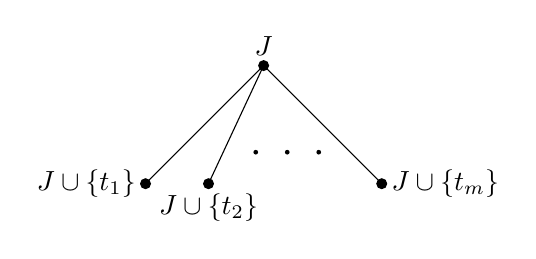
\begin{tikzpicture}
\fill (0,0) circle (.07);
\fill (.8,0) circle (.07);
\fill (3,0) circle (.07);
\fill (1.5,1.5) circle (.07);
\draw (1.5,1.5) - - (0,0) node[above, pos = 0]{$J$} node[left, pos = 1]{$ J\cup \{t_1\}$};
\draw (1.5,1.5) - - (.8,0) node[below, pos = 1]{$J \cup \{t_2\}$};
\draw (1.5,1.5) - - (3,0) node[right, pos = 1]{ $J\cup \{t_m\}$};
\fill (1.4, .4) circle (.03);
\fill (1.8, .4) circle (.03);
\fill (2.2, .4) circle (.03);
\end{tikzpicture}
\end{center}
\item Show that $Z(A)$ is a tree for any apartment $A$ of $\Delta$.

\end{itemize}
\end{frame}

\begin{frame}
\frametitle{Sketch continued}
To show that $Z(A)$ is a tree, we move between points in $Z(A)$ using galleries (paths between chambers) in the apartment $A$. The difficult part is to show that circuits cannot arise. 
\vskip .5cm
\begin{enumerate}
\item Choose $Z$ wisely so that the copies can only be glued together by panels with no relations between them (i.e. $Z_s$, $Z_t$ such that $m(s,t) = \infty$)
\vskip .3cm
\item Use a technical lemma about when words in a Coxeter group can be reduced to the trivial word to show that we can't get back to the starting point.
\end{enumerate}
\end{frame}


\begin{frame}
\frametitle{Sketch continued}
\begin{itemize}
\item If $Z(A)$ is a tree, then $Z(\Delta)$ is also a tree.\\
\smallskip
One can show this by using retractions (a building has a canonical retraction onto any apartment) or using the fact that if $Z(A)$ is $\CAT(0)$, then $Z(\Delta)$ is $\CAT(0)$.
\item Show that the cell stabilizers, which are intersections of parabolic subgroups, are finite and of unbounded order. 
\item Then $G$ acts on a product of two trees, one for each half of the twin building, which is a contractible 2-D space. Hence $G$ is not $\FP_2$. 
\end{itemize}
\end{frame}

\begin{frame}
\frametitle{Other results}
\begin{Theo}[G.]
Suppose $G$ acts strongly transitively on a locally finite twin building and has Coxeter system $(W,S)$ such that
$$
S = \coprod_{i=1}^n J_i, \; n\geq 2,
$$
where all the $J_i$ are spherical subsets of $S$ but $m(s,t) = \infty$ whenever $s\in J_i$ and $t\in J_j$ for $i\neq j$. Then $G$ is not $\FP_2$.
\end{Theo}

This also takes care of the case when all labels are infinite (in which case it is equivalent to the Davis realization). 
\end{frame}

\begin{frame}
\frametitle{Sketch of Proof}
Choose $Z$ to be the geometric realization of the flag complex on $\{\emptyset, J_1,\ldots, J_n\}$ and $Z_s$ the same for the subsets containing $s$:
\begin{center}
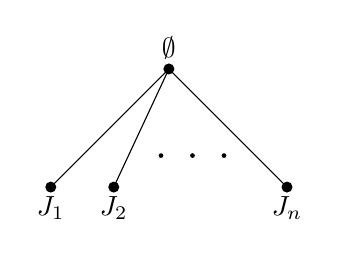
\begin{tikzpicture}
\fill (0,0) circle (.07);
\fill (.8,0) circle (.07);
\fill (3,0) circle (.07);
\fill (1.5,1.5) circle (.07);
\draw (1.5,1.5) - - (0,0) node[above, pos = 0]{$\emptyset$} node[below, pos = 1]{$ J_1$};
\draw (1.5,1.5) - - (.8,0) node[below, pos = 1]{$J_2$};
\draw (1.5,1.5) - - (3,0) node[below, pos = 1]{ $J_n$};
\fill (1.4, .4) circle (.03);
\fill (1.8, .4) circle (.03);
\fill (2.2, .4) circle (.03);
\end{tikzpicture}
\end{center}
The strategy is similar to the previous proof, but showing that no circuits exist is easier since 
$$
W = W_{J_1}*\cdots *W_{J_n}.
$$
\end{frame}

\begin{frame}
\frametitle{Rank 3 cases}
\begin{Theo}[G.]
Suppose that $G$ acts strongly transitively on a twin building and has rank $3$ Weyl group with at least one $\infty$ label in the associated Coxeter diagram. Then $G$ is not $\FP_2$ and is therefore not finitely presented.
\end{Theo}
\vskip 1cm
The first case of all $\infty$ labels is taken care of by the previous result.
\end{frame}

\begin{frame}
\frametitle{Rank 3, one $\infty$}
\begin{center}
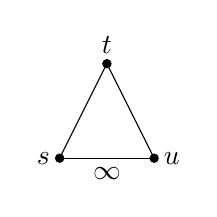
\begin{tikzpicture}[scale=1.2]
\fill (0,0) circle (.05);
\fill (1,0) circle (.05);
\fill (.5,1) circle (.05);
\draw (0,0) - - (1,0) node[pos = 0, left]{$s$} node[pos = .5, below]{$\infty$} ;
\draw (1,0) - - (.5, 1) node[pos = 0, right]{$u$};
\draw (0,0) - - (.5,1) node [pos = 1, above] {$t$} ;
\end{tikzpicture}
\end{center}

\begin{itemize}
\item $Z$ is the geometric realization of the flag complex on spherical subsets of $S$ containing $t$
\item $Z_t = Z$
\item $Z_s, Z_u$ are geometric realizations of flag complex on spherical subsets containing $\{s,t\}$ and $\{s,u\}$, respectively.
\end{itemize}
\vspace{4ex}

\begin{center}
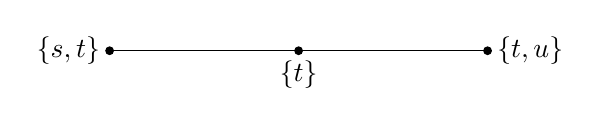
\begin{tikzpicture}[scale=.8]
\fill (0,0) circle (.07);
\fill (3,0) circle (.07);
\fill (6,0) circle (.07);
\draw (0,0) -- (3,0) node[pos = 0, left]{$\{s,t\}$};
\draw (3,0) -- (6,0) node[pos = 0, below]{$\{t\}$} node[pos = 1, right]{$\{t,u\}$};
\end{tikzpicture}
\end{center}
\end{frame}

\begin{frame}
\frametitle{Rank 3, two $\infty$s}
\begin{center}
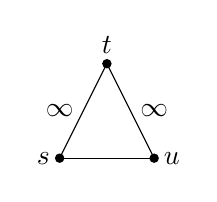
\begin{tikzpicture}[scale=1.2]
\fill (0,0) circle (.05);
\fill (1,0) circle (.05);
\fill (.5,1) circle (.05);
\draw (0,0) - - (1,0) node[pos = 0, left]{$s$} node[pos = 1, right]{$u$};
\draw (1,0) - - (.5, 1) node[pos = .5, right]{$\infty$};
\draw (0,0) - - (.5,1) node [pos = 1, above] {$t$} node[pos = .5, left] {$\infty$};
\end{tikzpicture}
\end{center}
Let $J_1 = \{s,u\}$ and $J_2 = \{t\}$ and use the second result.
\begin{itemize}
\item $Z$ is the geometric realization on the flag complex on $\{\emptyset, J_1, J_2\}$.
\item $Z_s, Z_t, Z_u$ are the geometric realizations on the flag complexes on the subsets containing $s,t,u$, respectively.
\item $Z_s = Z_u$
\end{itemize}


\begin{center}
\begin{tikzpicture}
\fill (0,0) circle (.07);
\fill (3,0) circle (.07);
\fill (6,0) circle (.07);
\draw (0,0) -- (3,0) node[pos = 0, left]{$\{s,u\}$};
\draw (3,0) -- (6,0) node[pos = 0, below]{$\emptyset$} node[pos = 1, right]{$\{t\}$};

\end{tikzpicture}
\end{center}
\end{frame}

\begin{frame}
\frametitle{Amalgamated product decomposition}
\begin{Prop}
If $G$ has Coxeter system $(W,S)$ such that there exist generators $s,t\in S$ such that $m(s,t) = \infty$, then $G$ acts on a tree with a segment as fundamental domain. Furthermore, if we name the edge $e$ with vertices $v$ and $w$, then $G = G_v *_{G_e} G_w$ is the amalgamated product of the vertex stabilizers over the edge stabilizer.
\end{Prop}

\begin{center}
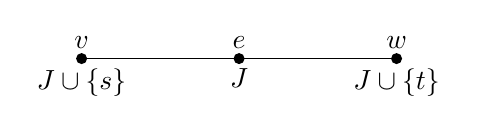
\begin{tikzpicture}
\fill (0,0) circle (.07);
\fill (2,0) circle (.07);
\fill (4,0) circle (.07);
\draw (0,0) - - (2,0) node[below, pos = 0]{$J\cup \{s\}$} node[below, pos = 1]{$J$} node[above, pos = 0]{$v$};
\draw (2,0) - - (4,0) node[below, pos = 1]{$J \cup \{t\}$} node[above, pos = 1] {$w$} node[above, pos = 0]{$e$};
\end{tikzpicture}
\end{center}
\end{frame}


%\begin{frame}
%\frametitle{Results}
%
%\begin{Theo}[G.]
%Suppose that $G = \cG(\FF_q)$ has rank $3$ Weyl group with at least one $\infty$ label in the associated Coxeter diagram. Then $G$ is not $\FP_2$ and is therefore not finitely presented.
%\end{Theo}
%
%All rank $3$ cases are taken care of with some generalizations as well. The key is to find the right $Z$ and $Z_s$ for the $Z$-realization for our group to act on.
%\end{frame}
%
%
%\begin{frame}
%\frametitle{Case 1}
%\begin{center}
%\begin{tikzpicture}[scale=1.2]
%\fill (0,0) circle (.05);
%\fill (1,0) circle (.05);
%\fill (.5,1) circle (.05);
%\draw (0,0) - - (1,0) node[pos = 0, left]{$s$} node[pos = .5, below]{$\infty$} node[pos = 1, right]{$u$};
%\draw (1,0) - - (.5, 1) node[pos = .5, right]{$\infty$};
%\draw (0,0) - - (.5,1) node [pos = 1, above] {$t$} node[pos = .5, left] {$\infty$};
%\end{tikzpicture}
%\end{center}
%
%In this case, we use the Davis realization, where $Z$ is defined as in the example above as the geometric realization of the flag complex on the set of spherical subsets of $S$.
%
%That is, $Z$ is 
%
%\begin{center}
%\begin{tikzpicture}[scale=.8]
%\fill (0,0) circle (.07);
%\fill (2,0) circle (.07);
%\fill (4,0) circle (.07);
%\fill (2,2) circle (.07);
%\draw (0,0) -- (2,0) node[pos = 0, left]{$s$} node[pos = 1, below]{$\emptyset$};
%\draw (2,0) -- (4,0) node[pos = 1, right]{$u$};
%\draw (2,0) -- (2,2) node[pos = 1, above]{$t$};
%\end{tikzpicture}
%\end{center}
%\end{frame}
%
%\begin{frame}
%\frametitle{Case 2}
%\begin{center}
%\begin{tikzpicture}[scale=1.2]
%\fill (0,0) circle (.05);
%\fill (1,0) circle (.05);
%\fill (.5,1) circle (.05);
%\draw (0,0) - - (1,0) node[pos = 0, left]{$s$} node[pos = .5, below]{$\infty$} ;
%\draw (1,0) - - (.5, 1) node[pos = 0, right]{$u$};
%\draw (0,0) - - (.5,1) node [pos = 1, above] {$t$} ;
%\end{tikzpicture}
%\end{center}
%
%\begin{itemize}
%\item $Z$ is the geometric realization of the flag complex on spherical subsets of $S$ containing $t$
%\item $Z_t = Z$
%\item $Z_s, Z_u$ are geometric realizations of flag complex on spherical subsets containing $s,t$ and $s,u$, respectively.
%\end{itemize}
%\vspace{4ex}
%
%\begin{center}
%\begin{tikzpicture}[scale=.8]
%\fill (0,0) circle (.07);
%\fill (3,0) circle (.07);
%\fill (6,0) circle (.07);
%\draw (0,0) -- (3,0) node[pos = 0, left]{$s,t$};
%\draw (3,0) -- (6,0) node[pos = 0, below]{$t$} node[pos = 1, right]{$t,u$};
%
%\end{tikzpicture}
%\end{center}
%\end{frame}
%
%
%\begin{frame}
%\frametitle{Case 3}
%\begin{center}
%\begin{tikzpicture}[scale=1.2]
%\fill (0,0) circle (.05);
%\fill (1,0) circle (.05);
%\fill (.5,1) circle (.05);
%\draw (0,0) - - (1,0) node[pos = 0, left]{$s$} node[pos = 1, right]{$u$};
%\draw (1,0) - - (.5, 1) node[pos = .5, right]{$\infty$};
%\draw (0,0) - - (.5,1) node [pos = 1, above] {$t$} node[pos = .5, left] {$\infty$};
%\end{tikzpicture}
%\end{center}
%
%This falls under a more general result:
%\begin{Theo}[G.]
%Suppose that $G$ has associated Weyl group generated by $S$ such that $S = \sqcup_{i=1}^n J_i$ where $n\geq 2$ and each $J_i$ is spherical but $m(s,t) = \infty$ whenever $s\in J_i, t\in J_j$ for $i\neq j$. Then $G$ is not $\FP_2$.
%\end{Theo}
%
%For this rank $3$ case, let $J_1 = \{s,u\}$ and $J_2 = \{t\}$.
%
%\end{frame}
%
%\begin{frame}
%\frametitle{Case 3}
%
%\begin{itemize}
%\item $Z$ is the geometric realization on the flag complex on $\{\emptyset, J_1, J_2\}$.
%\item $Z_s, Z_t, Z_u$ are the geometric realizations on the flag complexes on the subsets containing $s,t,u$, respectively.
%\item $Z_s = Z_u$
%\end{itemize}
%
%\vspace{.8in}
%
%\begin{center}
%\begin{tikzpicture}
%\fill (0,0) circle (.07);
%\fill (3,0) circle (.07);
%\fill (6,0) circle (.07);
%\draw (0,0) -- (3,0) node[pos = 0, left]{$s,u$};
%\draw (3,0) -- (6,0) node[pos = 0, below]{$\emptyset$} node[pos = 1, right]{$t$};
%
%\end{tikzpicture}
%\end{center}
%
%\end{frame}

\begin{frame}
\begin{center}
\huge{Thank you!}
\end{center}
\end{frame}






\end{document}
